% \documentclass[Japanese]{dicomopapers}
\documentclass[Japanese,noauthor]{dicomopapers}

\usepackage[dvipdfmx]{graphicx}
\usepackage{latexsym}
\usepackage{amsmath}
\usepackage{url}

\def\Underline{\setbox0\hbox\bgroup\let\\\endUnderline}
\def\endUnderline{\vphantom{y}\egroup\smash{\underline{\box0}}\\}
\def\|{\verb|}
\def\newblock{\hskip .11em plus .33em minus .07em}

\begin{document}

% 和文表題
\title{ディスプレイを用いて光電脈波センサに\\任意の脈波を計測させる手法の提案}
% 英文表題
% \etitle{DICOMO2021 Paper Format (optional)}

% 所属ラベルの定義
\affiliate{Rits}{立命館大学大学院情報理工学研究科}
\affiliate{JST}{科学技術振興機構さきがけ}

\author{藤井 敦寛}{ATSUHIRO FUJII}{Rits}[atsuhiro.fujii@iis.ise.ritsumei.ac.jp]
\author{村尾 和哉}{KAZUYA MURAO}{Rits,JST}[murao@cs.ritsumei.ac.jp]

\begin{abstract}
  %ウェアラブルデバイスに関する研究は活発に行われており,様々な形状,装着部位のデバイスが提案されている.ウェアラブルデバイスは自身の生体情報を記録するために利用される場合が多く,取得されたデータから身体異常を検知する手法などが提案されている.生体情報の中でも脈波データは感情推定などに利用されている.
  脈波センサは緑色のLEDを皮膚に照射して,血管を通して反射した光の変化から脈波を計測する光電式容積脈波記録法(PPG)と呼ばれる方式のものが一般的であり,スマートウォッチをはじめとする市販のウェアラブルデバイスに導入されている.脈波センサは機構の特性上,データの取得に血流を必要とするが,義手やウェアラブルロボットアームなど人工的な身体にスマートウォッチを装着する場合,血流が存在しないため正しいデータが取得できない.そこで,ディスプレイを用いて光電脈波センサに任意の脈波データを計測させる手法を検討する.本手法が実現すれば,身体と義手の接合部などで計測された脈波を入力することで,その値を義手に装着したスマートウォッチに読み取らせることが可能となる.本稿では心拍数に注目し,目標とする任意の心拍数を入力することでディスプレイを制御し,ディスプレイ上に装着したスマートウォッチで目標とする心拍数が取得できるか調査した結果について述べる.ディスプレイ描画プログラムとスマートウォッチアプリケーションを実装し,スマートウォッチと2台のディスプレイを使用して評価実験を行った.その結果,目標心拍数とスマートウォッチで計測された心拍数の誤差がDisplay Aで平均-1.8回,Display Bで平均-1.6回であり,全体で-3回以内と高い精度で心拍数を再現できた.
\end{abstract}

% 表題などの出力
\maketitle

% 本文はここから始まる
\section{はじめに}
\label{introduction}
健康管理への意識の高まりから,自身の生体情報を記録するウェアラブルデバイスが広く普及している.記録する生体情報は活動量や呼吸数,体温,心電位,血圧,視線などさまざまな情報があり,脈波や心拍数もそのひとつである.脈波や心拍数を取得するために用いられる脈波センサは,赤外線や赤色,550nm付近の緑色波長の光をLEDで皮膚に照射する.動脈の血中に存在する酸化ヘモグロビンがこれらの光を吸収する特性があり,心拍のタイミングで血流量が増加することで反射光の量が減ることを利用して,フォトトランジスタを用いて光量の変化を取得し,脈波を計測する.脈波データはこの反射光の変化の数値データであり,心拍数は脈波データに出現するピークを検出することで計測される.この脈波計測方式を光電式容積脈波記録法(PPG: Photoplethysmogram)と呼ぶ.スマートウォッチをはじめとする市販のウェアラブルデバイスの多くは,この方式を利用した脈波センサを搭載している.脈波は生体情報の中でも重要なデータの一つであり,脈波データを用いて呼吸数を推定する手法をHavriushenkoら\cite{respiratory_rate_estimation}が提案しているなど,脈波データを使用した研究は盛んである.\par

一方で当然ながら,義手やウェアラブルロボットアームなど人工的な身体には血流が存在しないため,スマートウォッチを生身の身体と同様に手首に装着しても生体情報を計測することはできない.通話やメッセージ,時計,決済などのスマートウォッチの機能や加速度センサやGPSなどのセンサは人工的な身体であっても生身と同様にスマートウォッチを装着すれば利用できるが,脈波の計測はできない.脈波を計測するために足首に無理矢理スマートウォッチを巻くと,時計などの他の機能のユーザビリティが低下する.現状で脈波を計測したいのであれば,脈波センサを追加で計測可能な身体部位に装着し,スマートフォンなどと通信をしてデータを収集する必要がある.手首で体温計測を行う場面を考えても,店員と客がアクリル板で仕切られてアクリル板に空けられた穴越しにやりとりする場面では,人工的な身体を穴から差し出して計測してもらうことはできない.生身の身体向けに提供されている便利で使いやすいインタフェース,見た目に美しいデザイン,社会に浸透しているプロトコルなどを人工的な身体でもそのまま利用できるならば,そのような社会が望ましいと考える.\par

本研究では,ディスプレイを用いて光電脈波センサに脈波データを計測させる手法を提案する.提案手法によって,義手やウェアラブルロボットアームなどの人工的な身体にスマートウォッチを装着する場合でも,身体と義手の接合部などで計測された脈波を入力し,手首に埋め込まれたディスプレイを制御することで,本人の脈波データをスマートウォッチに読み取らせることができる.さらに,スマートウォッチが提供する時計などの機能を生身の身体と同様に利用できる.また,人工的な身体にディスプレイを搭載するのみでスマートウォッチには手を加えないため,市販のスマートウォッチのデザイン,機能,重量などのさまざまな項目を比較して好きな機種を利用できる.このほか,遠隔地のロボットアバタに適用すれば,操作者の生体情報をアバタの身体でも計測できるようになる.本稿では,スマートウォッチに任意の心拍数を計測させることを目指す.\par

他方,提案手法の実現によって,光電脈波センサに任意の心拍数を計測させるのが可能であることが明らかになるため,悪意ある利用者が心拍数を偽って運動したふりをしたり,安静を続けているふりをすることもできると考えられ,光電脈波センサの脆弱性を明らかにする側面もある.提案手法を実現するデバイスが広く一般に実現可能となり,社会的影響が大きくなった場合は,現状の光電脈波センサの利用について議論する必要があると考えるが,本稿ではこの点については深く議論しない.

以降,\ref{sec:related}節で関連研究を紹介し,\ref{sec:method}節で提案手法の詳細を説明する.\ref{sec:evaluation}節で提案手法の評価を行い,\ref{sec:future_work}節で今後の計画を述べ,最後に\ref{sec:conclude}節で本研究をまとめる.



\section{関連研究}
\label{sec:related}
本節ではウェアラブルデバイスのセンシング,スマートウォッチの利用,脈波データの利用に関する研究を紹介する.

\subsection{ウェアラブルデバイスのセンシング}
Hamら\cite{smart_wristband}はスマートグラス用の入力デバイスとして,リストバンド型のデバイスを提案している.このデバイスはタッチパネルと慣性計測ユニットを搭載しており,タッチや手首をひねるなどのモーションで操作ができる.手首にデバイスを装着することで使用できるため,ユーザは動きを制限されず,自由度が高い.また,ポインティングにはタッチパネルを使用することで,入力の安定性を向上させた.
Hernandezら\cite{bioglass}は頭部装着型のウェアラブルデバイスである,Google Glassに内蔵された加速度センサ,ジャイロセンサ,カメラから脈拍数と呼吸数を認識する手法を提案している.
Nishajithら\cite{smart_cap}は,視覚障害者の状況認識を支援するウェアラブルデバイスとして,スマートキャップの設計と実装を行った.デバイスはRaspberry Pi 3,Raspberry Pi NoIR Camera V2,イヤホン,電源から構成される.Raspberry Pi NoIR(No Infrared) Camera V2とはRaspberry Piの赤外線カメラモジュールである.この赤外線カメラで得られる画像から検出された対象物について,イヤホンを通して音声で説明する.
これらはいずれも身体部位に装着するウェアラブルデバイスに関する研究であり,様々な形状のデバイスを用いた研究が行われている.\par

さらに,デバイスの装着部位も多岐にわたる.
Vahdatpourら\cite{localization_vahdatpour}は25人の被験者に頭部,胸部,両上腕,両前腕,腰部,両大腿部,両脛部の計10箇所に加速度センサを装着してもらい,日常行動下の加速度データを収集した.収集したデータからSVM(Support Vector Machine)を用いて,平均89\%の精度で装着部位を推定した.
Sztylerら\cite{localization_sztyler}は15人の被験者の頭部,胸部,左上腕,左手首,腰部,ズボンの左ポケット,左足首の計7箇所に加速度センサを装着し,様々な身体活動における加速度データを収集した.収集したデータからRandom Forestを用いて装着部位を推定し,平均89\%の精度を達成した.
Kunzeら\cite{localization_kunze}は6人の被験者の右手首,右目付近の側頭部,ズボンの左ポケット,左胸のポケットの計4箇所に加速度センサを装着し,歩行動作におけるデータを収集した.収集したデータからC4.5分類木を用いて装着部位を推定した.
また,筆者ら\cite{localization_yoshida}はウェアラブルデバイスで取得可能な生体情報である心電と脈波を利用し,特定の行動を装着者に行わせることなくウェアラブルデバイスの装着部位を推定する手法を提案している.\par

このように,ウェアラブルデバイスは様々な形状のものが提案されており,装着部位も広範囲であることから,活発な研究が行われている.


\subsection{スマートウォッチの利用}
ウェアラブルデバイスの中でもスマートウォッチは早くから市販化されていることもあり,多くの研究が行われている.
Spinsanteら\cite{accuracy_in_low_intensity}は低強度の身体活動時にスマートウォッチから取得される心拍数に注目し,その精度を計測している.
Senら\cite{eating_recognition}はスマートウォッチの加速度センサおよび,ジャイロセンサから得られるデータを使用して,手,箸,スプーンのいずれを使用して食べたかなどの食事行動を記録する手法を提案している.スマートウォッチ内蔵のカメラで食品画像を撮影し,画像識別を行うことにより食事内容も記録する.
Johnstonら\cite{smartwatch_walk_authentication}はスマートウォッチは常に同じ場所,同じ方向で身に着けるものであることに着目し,スマートウォッチの加速度センサやジャイロセンサから得られるデータを使用して歩行に基づく生体認証を行う手法を提案した.一般的にスマートフォンはズボンのポケットやハンドバッグに格納して所持することが多い.これらの場所に比べ,スマートウォッチを装着する手首では活動の情報が大きく現れる傾向にある.
Weissら\cite{smartwatch_activity_recognition}は食事行動などの手に基づく身体行動において,スマートウォッチがスマートフォンよりも効果的に行動を識別できることを示した.``飲む''という行動において,スマートウォッチでは93.3\%の精度で識別できるのに対して,スマートフォンでは77.3\%の精度しか得られなかった.
Iakovakisら\cite{oh_detection}はスマートウォッチを用いて,姿勢変化による血圧(BP)の低下を予測することを目的とする研究を行っている.起立性低血圧(OH)はめまいや失神を引き起こす可能性があるとされており,高齢者だけでなく若年層でも転倒のリスクがある.そこで,心拍変動データを取得することで起立性低血圧による転倒リスクを低減する数学的予測モデルを提案している.
Mauldinら\cite{smartfall}は市販のスマートウォッチから得られる加速度データを用いて転倒を検知するAndroidアプリケーション``SmartFall''を提案している.スマートウォッチはSmartFallを実行するスマートフォンとペアリングされており,SmartFallはデータのプライバシーを守りつつクラウドサーバと通信し,転倒の予測に必要な計算をリアルタイムに実行する.
Ciabattoniら\cite{smartwatch_stress_detection}は様々な認知タスク中の精神的ストレスをリアルタイムに検出する手法を提案している.市販のスマートウォッチで取得したガルヴァニック皮膚反応(GSR),RR間隔,体温(BT)を用いてストレスを分類する.\par

人工的な身体ではウェアラブルデバイスを装着しても生体情報を収集できないため,これらの応用を利用できない可能性がある.加速度センサやGPSなどのセンサを用いた手法は適用できるが,生体情報を利用する手法は適用できない.これに対して筆者らは人工的な身体であったとしてもウェアラブルデバイスの生体情報センサにデータを計測させることで,生身の身体と同様にこれらの応用を利用できるようにすることを試みる.


\subsection{脈波データの利用}
Havriushenkoら\cite{respiratory_rate_estimation}はニューラルネットワークを用いて脈波データから呼吸数の推定を行う手法を提案している.呼吸数を測定する場合には鼻腔内に設置した熱センサや伸縮性のある胸部ベルトなどを用いることが多い.しかしながら,これらの方法は睡眠の妨げとなる可能性がある.脈波データを使用する手法であれば,ウェアラブルデバイスへの実装が可能である.検証の結果,2.2呼吸/分以下の平均呼吸数推定誤差を達成した.
Hanら\cite{arrhythmia_detection}はスマートウォッチから取得された脈波データから心房期外収縮(PAC)および,心室性期外収縮(PVC)を検出する手法を提案している.
Goshvarpourら\cite{emotion_recognition_poincare}は単純な動的信号処理技術と統合手法から感情の変化を分類する手法を提案している.35人の被験者から安静時および,特定の感情を刺激するような音楽を聴いている状態で心電図と指の脈拍を収集した.ポアンカレプロットを使用した後にSVMを用いて幸福,悲しみ,安らぎ,恐怖の4つの感情に分類した.
Kajiwaraら\cite{pulse_order_picking}は多くの物流企業が手動でのオーダーピッキングシステムを採用しており,感情やエンゲージメントが作業効率やヒューマンエラーに影響を与えることに注目し,ウェアラブルデバイスで取得した行動や脈波から,運動強度の高い作業中における感情やエンゲージメントを予測する手法を提案している.脈波,眼球運動,動作を深層ニューラルネットワークに入力することで,感情やエンゲージメントの推定を行う.検証実験の結果,誤り率0.12以下の精度で予測できることを明らかにした.
Leeら\cite{fast_emotion_recognition}は脈波データによる感情認識の速度向上に関する研究を行っている.行動価(valence)と覚醒度(arousal)に基づいた2次元の感情モデルを採用し,1D CNN(1次元畳み込みニューラルネットワーク)を用いることで,1.1秒の脈波データから感情認識を行う.1D CNNを二値分類(行動価,覚醒度が高いか低いか)としてDEAPデータセットを用いて実験したところ,行動価では75.3\%,覚醒度では76.2\%の認識精度を達成した.\par

脈波データは身体の異常検知や感情推定ができるなど,重要な生体情報の一つである.市販のウェアラブルデバイスの脈波センサの多くは光電式容積脈波記録法を使用している.そのため,血流が存在しない人工的な身体にウェアラブルデバイスを装着する場合,脈波データは取得できない.筆者らは生体情報の中でも脈波データに注目し,人工的な身体でも生身の身体と同様の脈波データをウェアラブルデバイスに計測させる手法を提案する.



\section{提案手法}
\label{sec:method}
本節では提案手法の詳細を述べる.


\subsection{概要}
\label{subsec:overview}
提案手法は任意の心拍数を設定すると,ディスプレイの表示が変化し,ディスプレイ上に装着したスマートウォッチに指定された心拍数を計測させる.提案手法の処理の流れを\figref{fig:method}に示す.はじめに,ユーザはコンピュータに表示されているコンソールから取得したい心拍数を入力する.提案手法は入力された心拍数に応じてコンピュータに接続されたディスプレイの明暗を変化させる.そして,ディスプレイ上に装着されたスマートウォッチは入力された心拍数と同じ数値の心拍数を計測する.\par

\begin{figure}[!t]
  \centering
  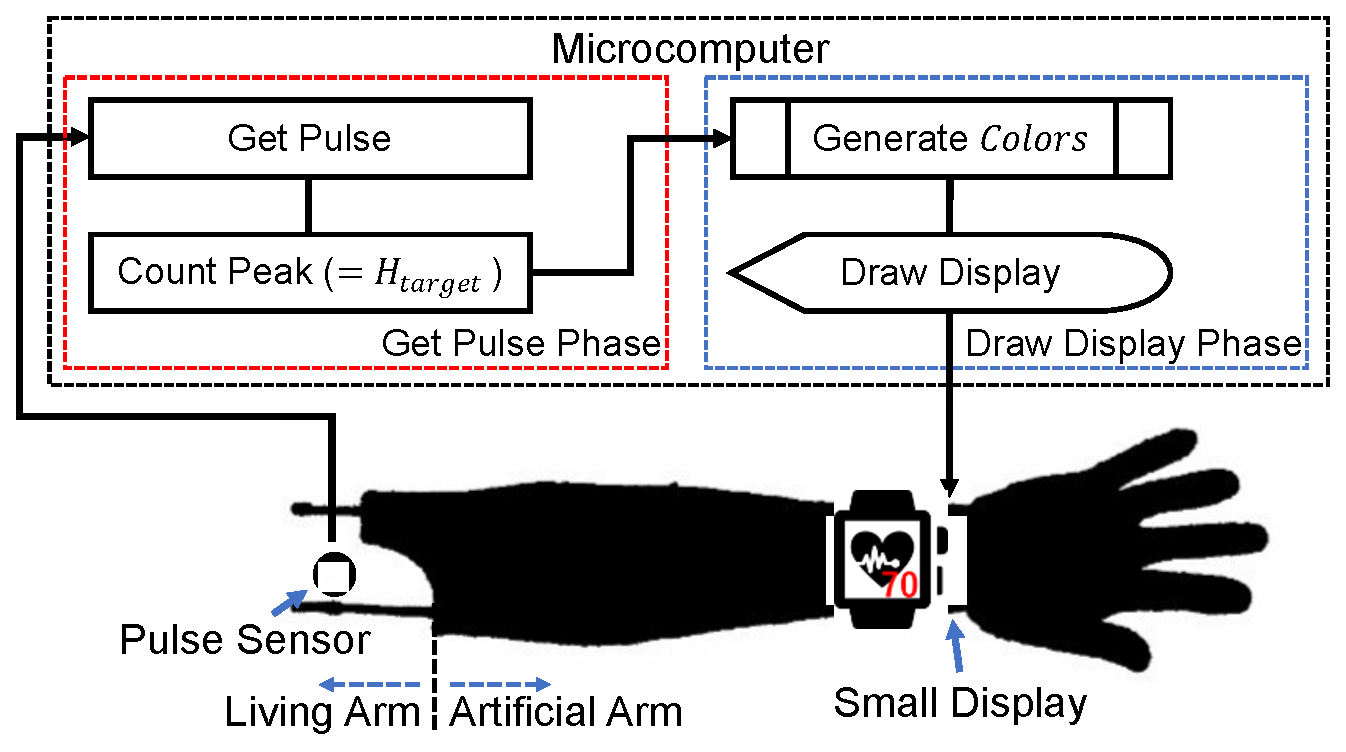
\includegraphics[width=1\linewidth]{figures/method.eps}
  \caption{提案手法の概要}
  \label{fig:method}
\end{figure}

\subsection{心拍数の設定}
本稿では提案手法によってスマートウォッチに計測させたい心拍数はディスプレイに接続されたコンピュータに明示的に与える設計としている.ただし,装着者の心拍数を別の心拍センサを利用して取得し,その数値を計測させたい心拍数としてリアルタイムに指定することもできる.設定された心拍数を$H_{target}$とする.

\subsection{ディスプレイの制御}
スマートウォッチが計測する心拍数が$H_{target}$となるように,ディスプレイの明暗を制御する.事前に,1回の脈拍をスマートウォッチに検出させることができるディスプレイの明暗の変化のデータ列$Colors$を用意する.ヒューリスティックに探索した事前調査から$Colors$は以下の数値列とした.
\begin{equation*}
  \begin{split}
    Colors = [255, 255, 255, 255, 255, 255, 255, 255, 255, 255,\\250, 240, 232, 227, 225, 225, 229, 236, 245, 255]
  \end{split}
\end{equation*}

$Colors$はグレースケールのデータである.グレースケールとはコンピュータでの色の表現方法の一種であり,黒から白までの色の濃淡を$0$ ~ $255$の256段階で表現する.具体的に$Colors$は以下の流れで生成している.
\begin{enumerate}
  \renewcommand{\labelenumi}{\arabic{enumi}.}
  \item $Colors[i]=\sin\left(\frac{2\pi i}{19}\right)~(i=0,\dots,19)$
  \item $Colors[i]=Colors[i]+1$
  \item $Colors[i]=1$ (if $Colors[i]>1$)
  \item $Colors[i]=Colors[i]*30+225$
\end{enumerate}
$Colors$をプロットしたものを\figref{fig:colors_wave}に示す.

光電式容積脈波記録法を用いた脈波センサは,赤外線や赤色,緑色のLEDを皮膚に照射して,血管を通して反射した光の変化から脈波を計測する.脈拍が発生するタイミングで血流量が増加するため,血管でより多くの光が吸収され,反射する光は暗くなる.\figref{fig:colors_wave}の値が低下している部分が反射光が暗くなる部分を表現している.グレースケールは値が小さくなるほど黒に近づく.黒は白に比べて光を吸収するため,ディスプレイが黒く描画されるほど,ディスプレイ上に装着したスマートウォッチから発せられてディスプレイを通して反射する光は暗くなる.

\begin{figure}[!t]
  \centering
  \includegraphics[width=1\linewidth]{figures/colors_wave.eps}
  \caption{スマートウォッチに1回の脈拍を検出させることができるディスプレイの明暗の変化のデータ}
  \label{fig:colors_wave}
\end{figure}

そして,1分間で$Colors$が$H_{target}$回だけ再生されるように,$Colors$の各値の描画間隔$T$[s]を以下のように設定する.
\begin{equation}
  \label{eqn:wait}
  T = 60 / (L_{Colors} * H_{target})
\end{equation}
ただし,$L_{Colors}$は$Colors$のデータ長(本稿では20)である.得られた$T$[s]ごとに$Colors$の値を1つずつ描画する.


\subsection{ディスプレイ描画プログラムの実装}
\label{subsec:software}
ディスプレイの明暗を変化させるプログラムをPythonとProcessingを用いて実装した.Processing\footnote{\url{https://processing.org}}とは視覚的な表現を得意とする,Javaをベースに開発されたプログラミング言語であり,電子アートやビジュアルデザインの作成などに使用される.実装したプログラムの処理の流れを\figref{fig:software}に示す.まず,Pythonで標準入力から目標とする心拍数$H_{target}$を受け取る.色データの作成部分ではNumpy\footnote{\url{https://numpy.org}}で$Colors$を作成する.そして,式(\ref{eqn:wait})を用いて$T$[s]を計算する.作成した$Colors$を1つずつPythonの\texttt{socket}ライブラリを使用してProcessingに送信し,描画の完了を待機する.Processing側ではデータを受信すると,そのグレースケールを\texttt{background}メソッドを使用して,ディスプレイに表示されているウィンドウの背景色として描画する.描画が完了したらPython側へ通知する.Python側で通知を受信すると現在時刻を取得し,あらかじめデータを送信する直前に取得しておいた$T_{now}$と比較を行い,$T$[s]が経過すると次の色データを送信する.この流れを繰り返し,$Colors$のデータを全て送信したら,再び$Colors$の1番目から同様にデータを取り出して処理を行う.

\begin{figure}[!t]
  \centering
  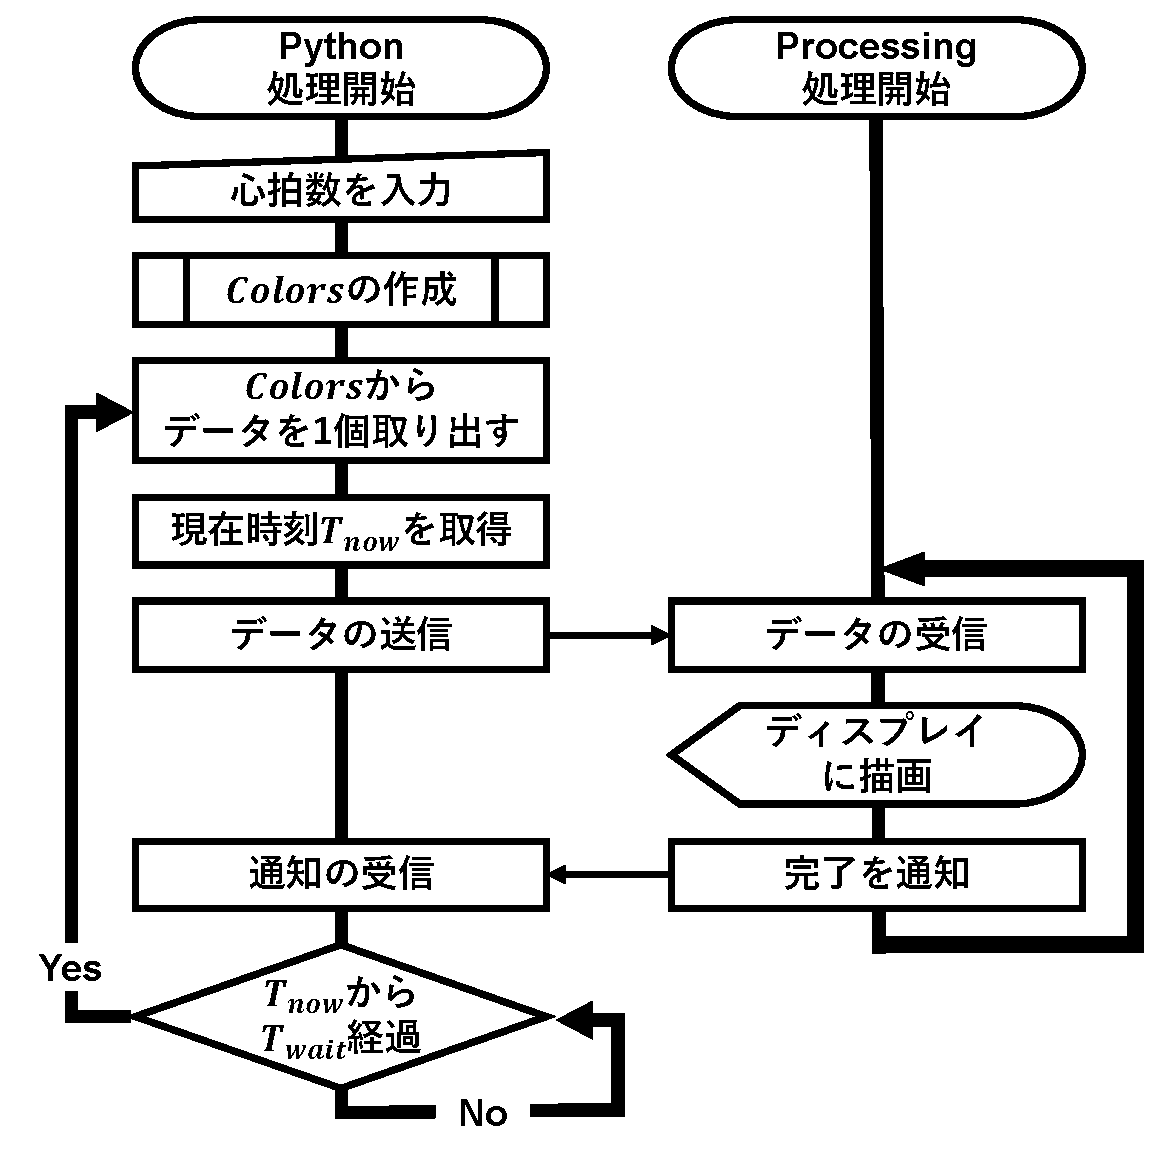
\includegraphics[width=1\linewidth]{figures/software.eps}
  \caption{実装したプログラムの処理の流れ}
  \label{fig:software}
\end{figure}



\section{評価}
\label{sec:evaluation}
本節では,提案手法の有効性を評価するために行った実験について説明する.任意の目標となる心拍数を与えた際にスマートウォッチで取得される心拍数を計測した.

\subsection{スマートウォッチアプリケーション}
\label{subsec:app}
評価実験ではスマートウォッチを利用して心拍数を計測するが,初期からインストールされているアプリケーションでは一定時間経過するとセンシングを停止して画面がOFFになったり,心拍数を数値として保存できないため,心拍数をロギングするスマートウォッチアプリケーションを実装した.

今回は評価実験にGoogleのAndroidをベースにスマートウォッチ向けに設計されたOSであるWear OS by Google\footnote{\url{https://wearos.google.com}}を搭載したスマートウォッチを使用するため,Android Studioで実装した.実装したアプリケーションを\figref{fig:app}に示す.アプリケーションを起動すると,図中(1)の画面が表示される.センサ値の取得が自動的に開始され,値に変化があった場合,(2)のようにセンサ値が表示される.``Heart''は心拍数センサ,``Pulse''は脈波センサの値を示す.データを記録する場合は``RECORD''ボタンを押下すると,(3)のように60秒間のキャリブレーションが開始される.このキャリブレーションは値の変動を安定させるために待機するものである.この間にスマートウォッチを固定しておく.60秒間のキャリブレーションが終了すると,(4)のように60秒間センサデータを取得し,変数に保存する.センサデータの取得時間が終了すると,変数に保存しておいたデータをcsv形式でスマートウォッチのストレージに保存し,(5)のように取得完了を示すメッセージが表示される.実装に使用したセンサの詳細について\tabref{tab:sensor_param}に示す.脈波データを取得するためのセンサ番号はデバイスにより異なる.ここでは評価実験に使用したTicWatch Pro WF12106(Mobvoi社製)でのセンサ番号を示す.サンプリングパラメータの``SENSOR\_DELAY\_UI''とは,ユーザインタフェースの実装に適したサンプリングレートである.\footnote{\url{https://developer.android.com/reference/android/hardware/SensorManager}}

\begin{figure}[!t]
  \centering
  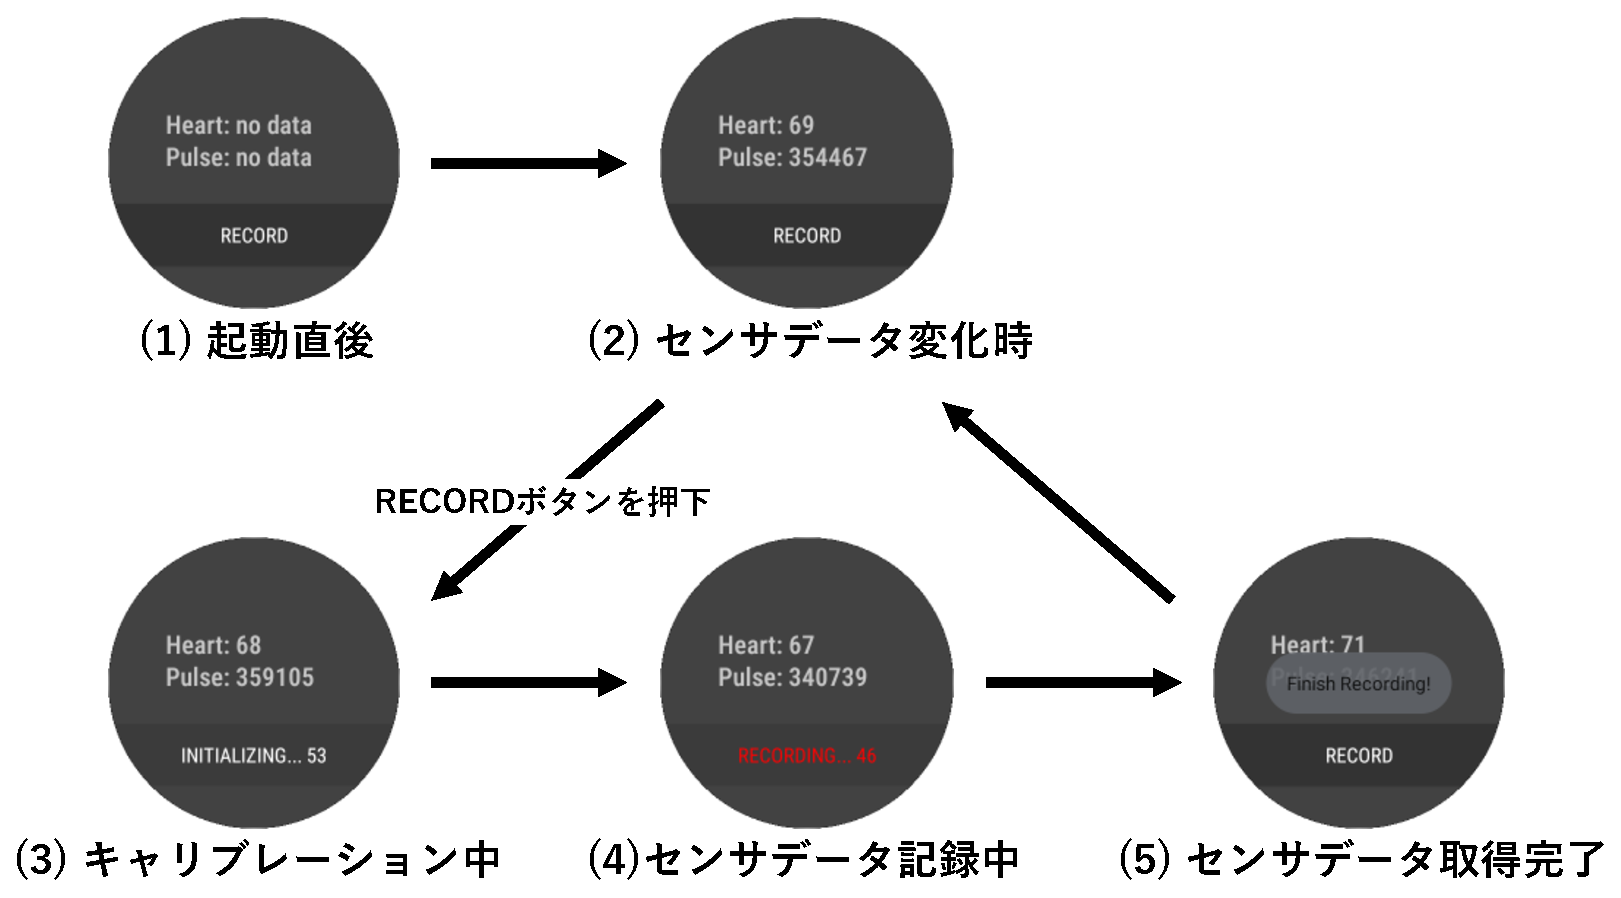
\includegraphics[width=1\linewidth]{figures/app.eps}
  \caption{実装したアプリケーション}
  \label{fig:app}
\end{figure}

\begin{table}[!t]
  \centering
  \caption{実装に使用したセンサの詳細}
  \begin{tabular}{c|c|c} \hline\hline
    取得対象 & センサ番号 & サンプリングパラメータ \\ \hline
    心拍数 & 21 & SENSOR\_DELAY\_UI \\
    脈波データ & 65572 & SENSOR\_DELAY\_UI \\ \hline
  \end{tabular}
  \label{tab:sensor_param}
\end{table}


\subsection{実験環境}
\ref{subsec:software}節で実装したディスプレイ描画プログラムと\ref{subsec:app}節で実装したスマートウォッチアプリケーションを使用してデータの収集を行う.スマートウォッチにはTicWatch Pro WF12106(Mobvoi社製)を使用し,ディスプレイはプログラムの実行に使用するノートPCであるLegion 7 15IMH05(Lenovo社製)の内蔵ディスプレイ(以下Display A)とマイクロコンピュータであるRaspberry Pi向けに設計された小型の3.5インチディスプレイ(OSOYOO社製)(以下Display B)を使用した.プログラムを実行するノートPCとDisplay Bの接続にはHDMIを使用した.また,Display Bには購入時に画面を保護するためのフィルムが貼り付けてあったが,剥がした場合は正しくセンサ値が取得できなかったことから貼り付けたままの状態で実験を行った.心拍数データ取得のサンプリングレートは約1Hz,脈波データ取得のサンプリングレートは約21Hzである.

データの取得は次の流れで行った.まず,実装したスマートウォッチアプリケーションを起動する.次にディスプレイ描画プログラムを実行し,適当な心拍数でディスプレイの描画を開始する.その状態でスマートウォッチをディスプレイに設置し,センサデータが更新されていることを確認する.このときの状態を\figref{fig:smartwatches}に示す.設置が完了したら,ディスプレイ描画プログラムの標準入力から目標心拍数を入力し,スマートウォッチアプリケーションの``RECORD''ボタンを押下する.60秒間キャリブレーションした後に,60秒間データ取得が行われる.目標心拍数を成人の平均心拍数である60回から100回\cite{heart_rate_average}まで5刻みで増加させながらデータを取得していき,100回に達すると再度60回から取得を繰り返す流れを3セット行う.以上の流れでディスプレイ2台でデータの取得を行った.

\begin{figure}[!t]
  \centering
  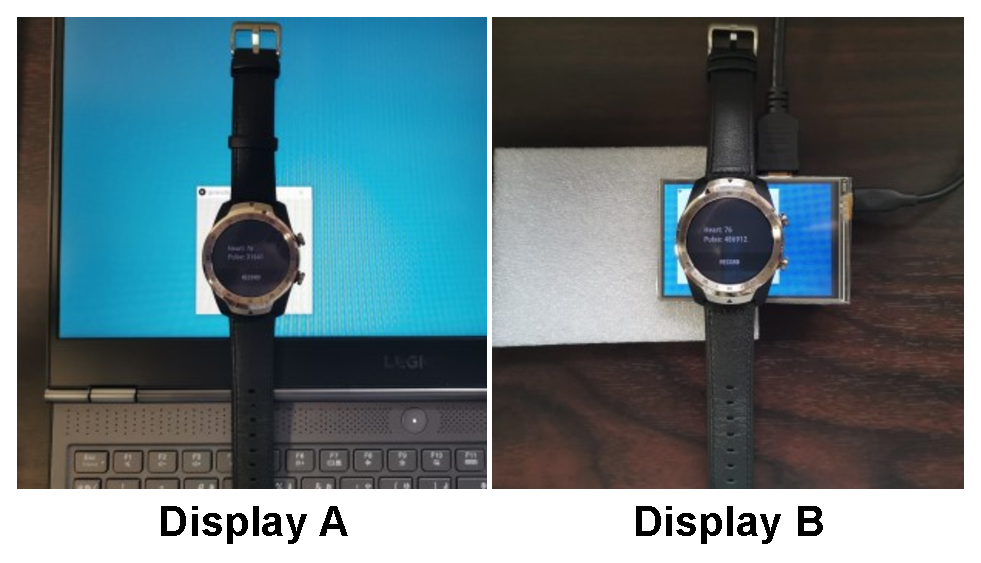
\includegraphics[width=1\linewidth]{figures/smartwatches.eps}
  \caption{評価実験での心拍数の取得方法}
  \label{fig:smartwatches}
\end{figure}


\subsection{結果と考察}
設定した目標心拍数とスマートウォッチで取得された心拍数の誤差を\tabref{tab:heartrate}に示す.この結果は3セットの平均値である.0は目標心拍数と一致していることを示し,マイナスは回数が不足していることを示す.また,``Average''はディスプレイごとの誤差の平均値である.結果より,成人の平均心拍数である60回$\sim$100回において,目標心拍数より0$\sim$-3回以内の誤差でスマートウォッチに心拍数を入力できていることが確認できた.平均値ではあるが,目標心拍数を70回としたとき,Display Bを使用してスマートウォッチに心拍数を正しく入力できた.全体の平均としては目標心拍数よりDisplay Aでは1.8回少なく,Display Bでは1.6回少ないという結果となった.\par

\begin{table}[!t]
  \centering
  \caption{設定した目標心拍数とスマートウォッチで取得された心拍数の誤差}
  \begin{tabular}{c|c|c} \hline\hline
    目標心拍数 & Display A & Display B \\ \hline
    60 & -1.0 & -1.0 \\
    65 & -1.3 & -1.3 \\
    70 & -1.0 & 0.0 \\
    75 & -2.0 & -1.7 \\
    80 & -2.0 & -2.0 \\
    85 & -2.0 & -2.3 \\
    90 & -2.0 & -2.0 \\
    95 & -2.0 & -1.7 \\
    100 & -2.7 & -2.3 \\ \hline
    Average & -1.8 & -1.6 \\ \hline
  \end{tabular}
  \label{tab:heartrate}
\end{table}

目標心拍数が大きくなるほど,スマートウォッチで取得される心拍数はマイナス方向への誤差が大きくなっている.これは処理時間の同期の精度の低さや,ディスプレイのリフレッシュレートが関係していると考えられる.\figref{fig:method}のとおり,提案手法では$T$[s]ごとに色を更新していく必要があるが,PythonとProcessingでデータのやり取りなどもする必要があり処理時間により遅延が生じてしまい,本来ディスプレイに60秒間で描画すべき回数よりも描画回数が少なくなってしまっている可能性がある.この遅延時間は,処理回数の増加にともなって増加すると考えられる.そのため,目標心拍数が大きくなるほど処理回数が増加し,ディスプレイへの描画の遅延が増加してしまい右肩下がりの傾向になったと考えられる.また,リフレッシュレートが低いと,正しく全ての色を$T$[s]ごとに描画できない可能性がある.リフレッシュレートについては,ディスプレイの性能に依存する.



\section{今後}
\label{sec:future_work}
評価実験ではディスプレイを用いてスマートウォッチに-3回以内の精度で,目標とする心拍数を計測させることができた.しかしながら,ディスプレイに対する制約が存在するほか,装着位置によっても取得される値がシビアに変化してしまう可能性が考えられる.今後は,実環境での使用を想定して脈波データの再現性を高めつつ,身体部位から得られた実際の脈波データを入力することで,ディスプレイ上に装着したウェアラブルデバイスに同一の脈波データを計測させる機構を実装する.この機構の想定を\figref{fig:future_work}に示す.実現するには,ディスプレイに描画する色を自動で決定し続ける必要がある.そのため,脈波データを入力することでディスプレイに描画する色を出力することができるような生成モデルを構築していく.また,身体部位に装着して使用することを想定し,デバイスの小型化を進めていくほか,複数のウェアラブルデバイスを使用して実験を行っていく.

\begin{figure}[!t]
  \centering
  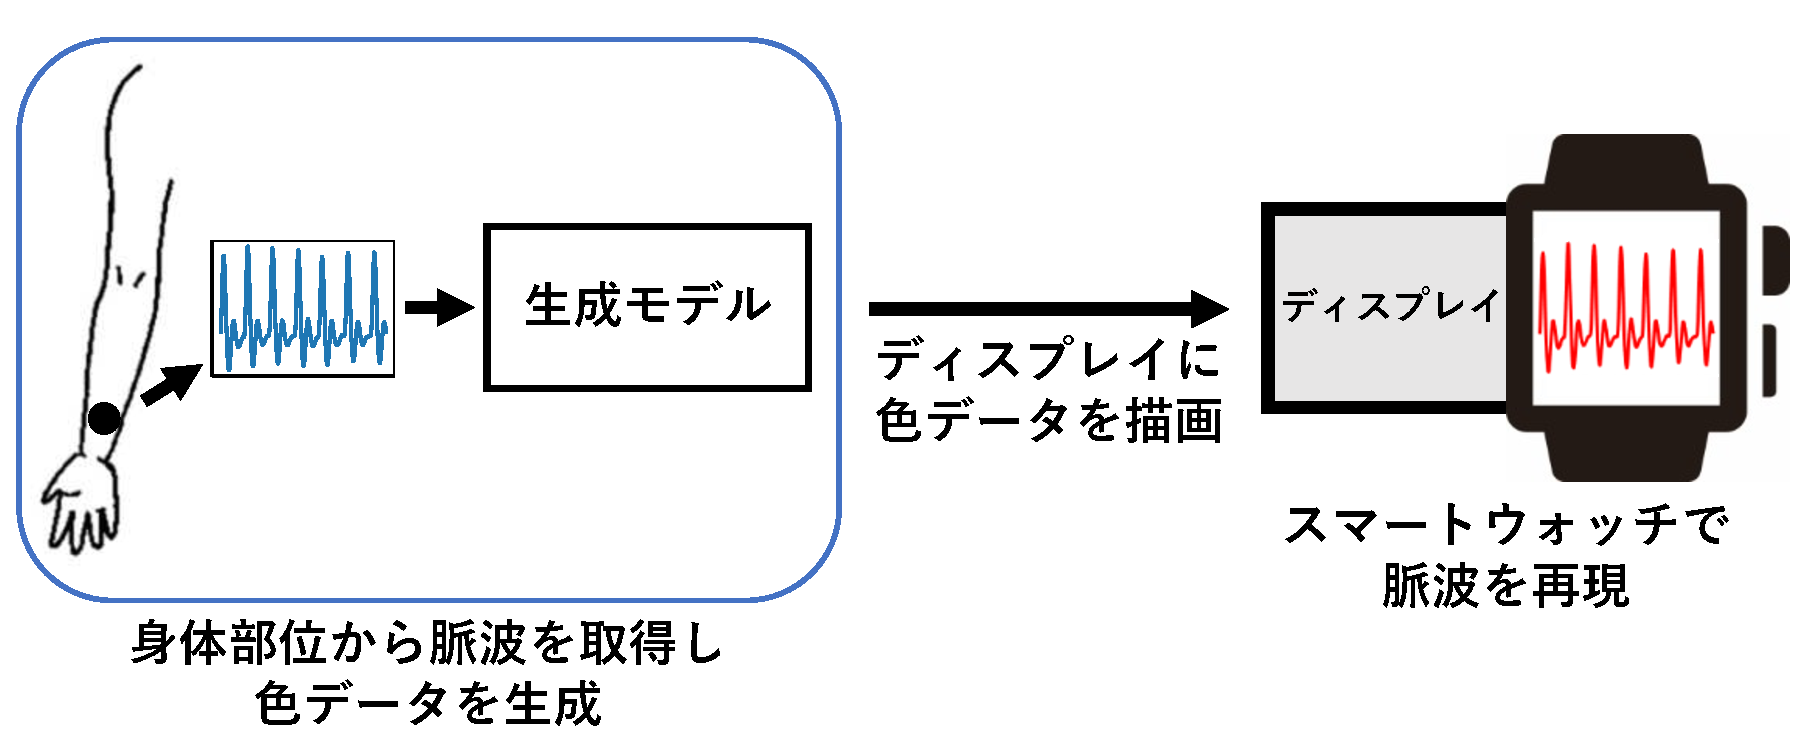
\includegraphics[width=1\linewidth]{figures/future_work.eps}
  \caption{身体部位から得られた脈波データを入力して再現する機構}
  \label{fig:future_work}
\end{figure}


\section{まとめ}
\label{sec:conclude}
本研究では,ディスプレイを用いて光電脈波センサに任意の心拍数を計測させる手法を提案した.ディスプレイ描画プログラムおよび,スマートウォッチアプリケーションを実装し,スマートウォッチとディスプレイ2台を使用して,提案手法の効果を確認するための評価実験を行った.その結果,入力した目標心拍数と実際にスマートウォッチで取得された心拍数の誤差が全体で-3回以内だった.ディスプレイごとの平均はDisplay Aで-1.8回,Display Bで-1.6回という結果であり,高い精度で心拍数が再現できた.\par

今後はディスプレイを用いることで,身体部位から取得された実際の脈波データと同様の脈波データをウェアラブルデバイスに計測させる機構を実装する.そのためには,自動でディスプレイの色調を決定していく必要があるため,適切な生成モデルを設計していく.また,身体部位への装着を想定し,デバイスの小型化を検討していく.



\begin{acknowledgment}
  本研究は,科学技術振興機構戦略的創造研究推進事業さきがけ(JPMJPR1937)の支援を受けたものである.ここに記して謝意を表す.
\end{acknowledgment}


\bibliography{references}
\bibliographystyle{junsrt}

\end{document}
